\documentclass[a4paper]{article}
\usepackage{graphicx}
\usepackage{onecolceurws}
\usepackage{csquotes}
\usepackage{hyperref}
\usepackage{framed}
\usepackage{mdframed}
\usepackage{upquote}
\usepackage{lmodern}
\usepackage[normalem]{ulem}

\newcommand\todo[1]{\textcolor{red}{TODO: #1}}

\title{Sophize Markdown and Collaboration Interface }

\author{ Abhishek Chugh }

\graphicspath {{../res}}

\institution{ Sophize Foundation\\ Bengaluru, India \\ abc@sophize.org }

\begin{document}
\maketitle

\begin{abstract}
Sophize is a novel mathematics library and discussion platform with a mission to help our users find and organize mathematical proofs. We present a Sophize's novel yet familiar knowledge organization scheme that is used to represent a wide variety proofs. With this knowledge organization scheme at its core, we have engineered that platform to aggregate knowledge from sources. The platform meaningfully combines knowledge from published research, encyclopedias such as PlanetMath and Wikipedia, informal computer programs and formal systems such as Metamath; and allows its users to run a federated search over them. To make this happen, two developments were necessary. First, we developed an open plugin architecture that allows proofs from computer programs to be generated as required. Second, we extended the Markdown language to represent the connections between between mathematical objects found across various sources of knowledge. In addition, we also utilized this new language to create a novel communication system built specifically to aid mathematicians in solving problems collaboratively.

\end{abstract}

\vskip 32pt

\section{Introduction [FROM CICM]}

\subsubsection*{Background: The Sophize Platform}

Sophize is a novel mathematics library and discussion platform. The author has developed the platform over the course of the last two years at \url{https://sophize.org}. Sophize's primary mission is to help users find existing proofs of mathematical statements, to discover new proofs, and to utilize this knowledge in their work. We combine knowledge from multiple resources and have accumulated thousands of definitions, theorems, and proofs from a wide variety of sources, including some published research, the PlanetMath encyclopedia, Wikipedia, and the Metamath formal system \cite{metamath}.

\todo{- The goal is rational truth. Three dimensions are consistency, correspondence and values.}

\todo{- In its current iteration, Sophize can model vast majority (almost all)  of mathematics.}

\subsubsection*{Proofs in Sophize}

Mathematical proofs are based on a variety of foundations such as ZFC, intuitionistic logic, and type theory. The arguments used in any proof are considered valid or not based on criteria that can vary. Most academic mathematics is peer-reviewed and published, but some mathematical proofs can be found in community curated sources such as Wikipedia. Proofs can also be algorithmically generated, and at the highest level of verification, they are represented and verified using a formal system. 

Sophize combines such an expansive range of proofs into a dense graph of propositions and logical arguments that aggregates knowledge from several documents and other data sources. We use this graph and combine it with the set of foundations and verifications chosen by each user to create proofs tailored to their needs. This introductory video gives an overview of the platform's offerings: \url{https://youtu.be/Wb1JbW9Otek}.

\begin{figure}[ht]
\begin{center}
\fbox{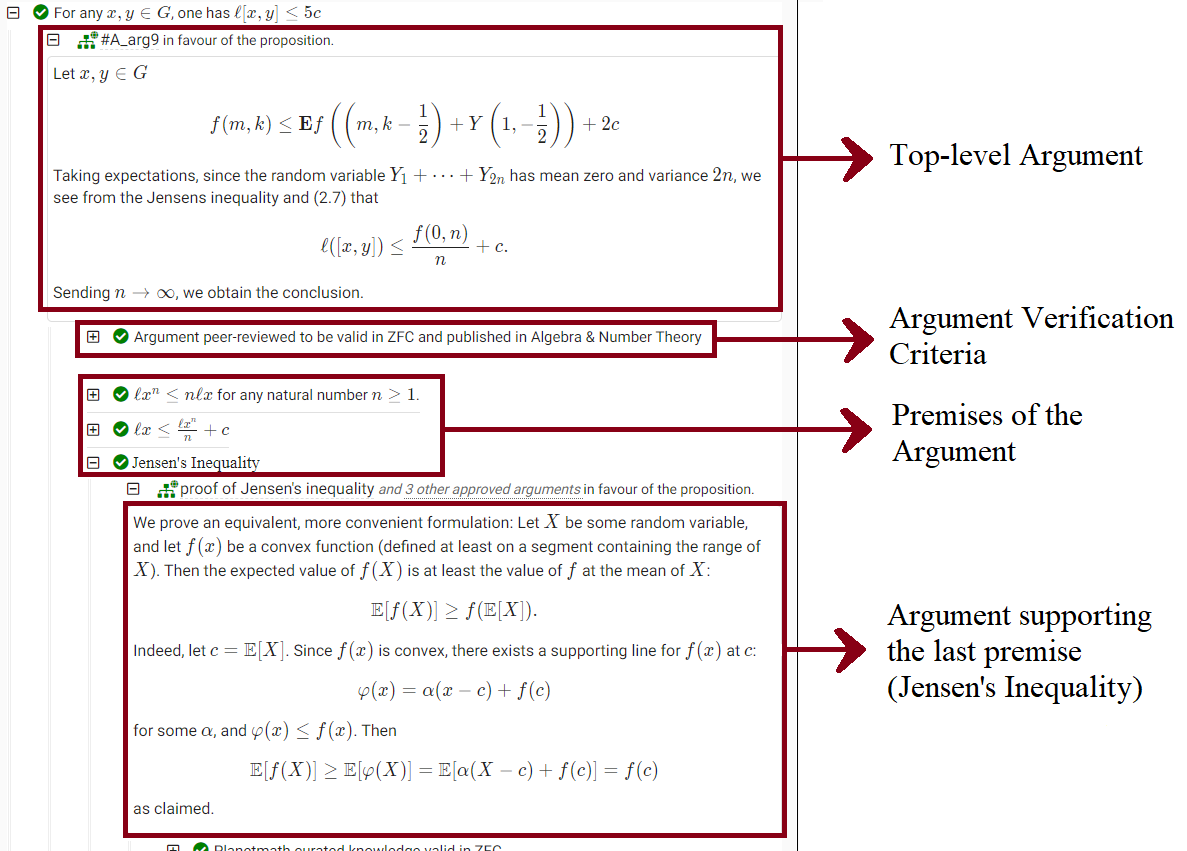
\includegraphics[height=12cm]{proof_tree}}
\caption{A proof displayed as a graph (tree) of arguments and propositions on the Sophize platform.}
\label{proof_tree}
\end{center}
\end{figure}

This work can also be seen as a step towards formalizing the network of information that exists in the connections of mathematical objects. The committee on planning a global library of the mathematical sciences recognized that this network is largely unexplored, and formalizing it has tremendous potential to accelerate math research \cite{sciences2014developing}.

Hence, we required novel knowledge organization techniques to connect mathematical entities from such a wide range of formal and informal knowledge sources. And thus, one of the main challenges towards building the Sophize platform was to create a simple way to embed mathematical entities on the web. \todo{Explain and summarize the problem statement}


\subsubsection*{Contribution}
\todo{summarize sections. section 3 does X, section 4 does Y etc.}

\subsection*{Acknowledgements}
This publication resulted (in part) from research supported by the International Mathematical Union. The author would like to thank Patrick Ion and Michael Kohlhase for help in organizing our ideas and structuring the content of the paper.

\section{Sophize's Knowledge Organization Scheme}
For math, logical consistency is the sole criteria for truth. Thus, as a math library, Sophize models mathematical knowledge using logical arguments. 

The various concepts used for organizing knowledge logically are described below. These concepts have been modelled in JSON schema \cite{sophize_datamodel} and published for popular programming language such as Java (MVN), Javascript (npm) and Python (PyPI). 

\paragraph{A \textbf{term} is a clearly defined entity that can be used to make up a valid proposition. It can be a mathematical object, operator, symbol, data structure, algorithm, or even a person. `Meaningless' primitives in formal theories are also categorized as terms.}

\paragraph{A \textbf{proposition} is a grammatically valid statement that can be either true or false. Axioms, theorems, conjectures, hypotheses, lemmas, corollaries, and converses are all classified as propositions.}

\paragraph{An \textbf{argument} is a set of propositions called premises along with a concluding proposition that is claimed to follow from the premises. In addition, most arguments include supporting text that explains how the conclusion follows from the premises. A proof is seen as a directed graph of arguments and propositions.}

\paragraph{A \textbf{resource} is an abstract concept inherited by all other top-level concepts like terms, propositions, and arguments. Each resource has a URI and contains fields such as search tags and citations.}

A \textbf{URI} consists of two parts: a namespace-like identifier called its dataset-id, which indicates the data source, and a resource-id that specifies the resource type and its unique name in the data source. The dataset-id may be omitted if it can be inferred from the surrounding context.

For example, the Pythagorean theorem (a \textbf{P}roposition) represented in the Metamath project may have the URI \emph{metamath/\textbf{P}\_pythagorean} and the definition of cone (a \textbf{T}erm) extracted from Wikipedia may have the URI \emph{wiki/\textbf{T}\_cone}. When used inside another resource in the `wiki' dataset, cone's definition can be referred to simply as \emph{T\_cone}.

The same URI scheme will be used in this paper to refer to various terms, propositions, arguments, etc.

There are a couple more concepts that we will describe at later in the paper.


\subsection{Validity of arguments}
Validity of an argument is, in principle, objectively verifiable. A formally defined logistic systems have a mechanical procedure to verify validity arguments.

However, mathematics only utilizes a tiny portion formally verifiable arguments. Most mathematics is verified via peer review, some of this knowledge is curated by experts in books, encyclopaedias. The claim of validity of proofs (arguments) is judged based on the various parameters such as academic standing of the claimant, reputation of the peer reviewing journal, the history of errors of the book or encyclopedia containing them, etc. Clearly, this criteria is subjective and can vary to some extent for each individual.

Sophize doesn't promote or endorse and such criteria. Instead, it allows its users to choose the criteria they believe in. A validity criteria is modelled as a proposition and each argument has one such validity criteria associated with it.

Some sample validity criteria:
1. Formally verified using 3 independent COQ verifiers.
2. Peer reviewed by XYZ journal
3. Published on Wikipedia.
4. Claimed by someone.

For easily managing validity criteria, the relationships between validity criteria are also maintained using arguments.
Eg. published in journal with score more than 0.67 $\rightarrow$ published in Annals of Mathematics


\todo{Q. Who has the time to setup belief sets? How does Sophize make it 
convenient.}


\subsection{Belief sets}

In Sophize, a proposition is claimed to be true if it is concluded by a valid argument and the premises of the argument are also true.

Of course, this means that we need to start with some propositions that are assumed to be true without further justification. Traditionally, these are mathematical axioms and are considered to self-evidently true. However, there is no clear criteria to claim if a propositions is self-evidently true. In mathematical inquiry, theorems are proven/disproven in one or more multiple theories, each with its own set of axioms. Each theory may have its theoretical advantages and practical uses and there are no criteria to choose one theory over another when trying to assert a proposition's truth/falsity.

Thus, Sophize allows any set of propositions to be considered true without evidence. Such a set of propositions is called a belief set. Thus, the truth-value of a proposition is only defined within a belief set - there is no notion of of absolute or universal truth. 

Propositions representing argument validity criteria are also part of belief sets. All propositions that are considered to be true in a belief set without proof are called `unsupported propositions'.

Computing of truth values in a belief set is thus a simple recursive graph algorithm as explained in the section below. Sophize computes truth values for all its belief sets.

\subsection{Tracking Inconsistency}
If a propositions and its negation is proved within a belief set is inconsistent. Due to principle of explosion, any propositions can be proved from such a contradiction. Thus making the claim of truth of any proposition practically worthless.

Thus it is important to track and report contradictions in a belief set. Thus Sophize has a semantic notion of negation of a proposition. The premises or conclusion of an argument can be negation of propositions.

When a proposition and its negation are proven, the system reports such contradictions for every belief set.

\subsection{Argument Graph}
A proposition is considered true if it is claimed by a sound argument. An argument is considered sound if it is valid and its premises are true. Also, as explained in the section above, the validity criteria of an argument is modelled as just another premise. Thus, the relationship between all propositions and arguments can be represented with a simple graph. The following figure shows the different types of nodes and edges in such a graph

1. Nodes - propositions and arguments
2. Edges - premise to argument and argument to conclusion

\subsection{Truth value computation}

Using the argument graph, we can find truth values of every proposition in a belief set. Starting with the unsupported proposition of the belief set, computing truth values can be done using a simple recursive algorithm. The output of this algorithm is another graph, that we call proof graph, that has a proof for all the propositions it contains. For each proposition, a proof in the form of DAG of arguments (starting with unsupported propositions) can be trivially extracted from this proof graph.

Note that an argument graph combines with different belief sets to generate different proof graphs. The same argument may be utilized in multiple belief sets.

\todo{alternate arguments, proofs for same proposition}

\subsection{Translations}
\todo{What are Translations? (informal to formal, formal to other formal), Why do we need translations?}

There is no good way to claim equivalency of propositions across different formal systems. [Formal Harmony still in infancy, theory morphisms aren't yet practical].


Eg. ZFC (informal) + ZFC (metamath) + Jensen's Inequality (metamath) + validity criteria (translation feels right to metamath group) $\rightarrow$ 
Jensen's Inequality (informal)

But, can represent translations manually using arguments. Such translations do not stand on a very firm foundation and that should be indicated in the validation criteria of the argument. Again, a user can choose not to accept this criteria in which case, these translations will not be used in the generating proof graphs.


Thus we can create proof graphs that have arguments from different languages.

\subsection{Uses}
Efficiently modelling different axiomatic systems that have a large overlap of arguments(eg. euclidean/parabolic/hyperbolic geometry, ZF/ZFC etc)

Conjectural knowledge (Reimann hypothesis). 
Practical utility of conjectural knowledge - eg. a lot of infromation security systems assume  P not NP)

\subsubsection{Other Notes}
\todo{How much math can be represented and Sophize's limitations. Eg. three valued logic}


\section{Proof Generating Automata}
A lot of mathematical knowledge is computed. Computations can be seen as algorithms that finding propositions based on some input.

The computation 15+16 results in the value 31. We see this as 


\section{Other Engineering challenges}
\todo{copyright/access management}
\todo{efficient computation and storage of proof graphs}
\todo{reading from disk }


\section{Sophize Markdown[FROM CICM]}

Markdown is a lightweight markup language for creating formatted text using a plain-text editor. Markdown is very widely adopted on the web, and it makes it quite simple to add lists, headers, bold or italic fonts, images, and more. One can choose from several slightly varying Markdown specifications. We start with the widely supported CommonMark specification and create extensions for the features that we need. The extensions are implemented using the `markdown-it' \cite{markdown_it} JavaScript parser. The parser for Sophize Markdown produces an abstract syntax tree (AST). A separate renderer module utilizes the AST tree to create the appropriate HTML or Single Page Application (SPA) libraries. Many of the features of Sophize Markdown are demonstrated at: \url{https://youtu.be/5UYOpQwcjCk}

\subsection{Embedding structured data}

With Sophize Markdown we can easily embed resources such as terms, propositions, and arguments. Links can be added using the resource's URI, and the following formats are supported:


\begin{itemize}

	\item \#URI[ $\vert$ OPTIONS ]

	Examples: \#wiki/T\_cone, \#planetmath/P\_covering\_lemma$\vert$NO\_LINK$\vert$LC

	\item \#(URI, \textquotesingle Custom\ Text\textquotesingle [ $\vert$ OPTIONS ])

	Examples: \#(wiki/T\_cone, \textquotesingle cones\textquotesingle), \#(P\_green\_tao\_theorem, 'Green–Tao Theorem'$\vert$NAV\_LINK)

\end{itemize}

There are multiple resource link options to embed a resource in the Markdown. These are required to make it convenient for the content creators to provide a rich experience to their readers. Some of the commonly used options are summarized below.

\subsubsection{Link Text Options}

\paragraph{\textbf{NAME} (default): This option fetches the resource and sets the link text to the name of the resource. For terms, the link text is set to the phrase of the term.}

\paragraph{\textbf{LOWER\_CASE (LC) or UPPER\_CASE (UC)}: These options become quite useful when adding a link in the beginning or middle of a sentence where adding the name in its default case would be grammatically incorrect.}

\paragraph{\textbf{Custom text}: A link can also explicitly specify the link text by enclosing it in single quotes.}

The following example shows the above options in use. Note that we assume that the dataset-id of URIs is available from the context and thus not specified in the URIs.

\begin{verbatim}
#P_cosine_law|UC is a generalization of the #P_pythagorean for all kinds of
#(T_triangle, 'triangles').
\end{verbatim}

\paragraph{The above code is rendered as:}
\begin{mdframed}
\dashuline{Law of cosines} is a generalization of the \dashuline{Pythagorean theorem} for all kinds of \dashuline{triangles}.
\end{mdframed}

\subsubsection{Link Type Options}

\paragraph{\textbf{OVERLAY\_LINK} (default): By default, clicking on links opens up a modal dialog with the resource's summary.}

\paragraph{\textbf{NAV\_LINK}: We can create a hyperlink to the resource's URL using the using NAV\_LINK option.}

\paragraph{\textbf{NO\_LINK}: NO\_LINK creates a non-clickable element whose hover text is the URI of the resource.}


For example, the following Markdown code has all three link types:
\begin{verbatim}
#T_matrix_multiplication|NO_LINK is a #(T_commutative_property, 
'non-commutative'|NAV_LINK) #T_binary_operation.
\end{verbatim}

\paragraph{The above code is rendered as:}
\begin{mdframed}
Matrix multiplication is a \underline{non-commutative} \dashuline{binary operation.}
\end{mdframed}
The first element shows `\#wiki/T\_matrix\_multiplication' on mouse-hover. The second link navigates the page to a different URL. Clicking on the third link pops up a modal dialog box like so:

\begin{figure}[ht]
\begin{center}
\fbox{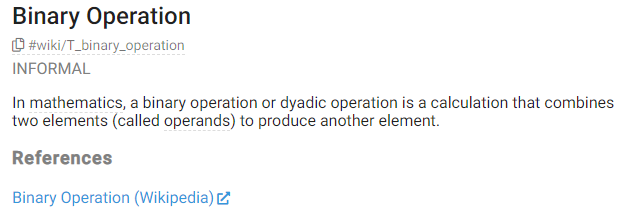
\includegraphics[height=5cm]{modal}}
\caption{Modal dialog box for the term binary operation. These boxes can also have content that uses all three types of links. }
\label{modal}
\end{center}
\end{figure}

\subsubsection{Resource Expansion}

Instead of creating a link, this option expands the resource in place. For terms and propositions, the definition and the statement are added in place, respectively. For arguments, its premises, conclusion, and the argument text is added.

The following is a sample article where we re-use concepts and theorems already extracted from multiple sources (say, Wikipedia and the Oxford dictionary):

\begin{verbatim}
# Conic section

A conic section (or simply conic) is a curve obtained as the intersection of the
#(wiki/T_conical_surface, 'surface') of a #wiki/T_cone with a #wiki/T_plane. There are
three types of conic sections.

## Ellipse
#oxford/T_ellipse|EXPAND #wiki/P_ellipse_area|EXPAND

## Parabola
#oxford/T_parabola|EXPAND The area of a parabola is unbounded.
...
\end{verbatim}

\paragraph{The above code is rendered as:}
\begin{mdframed}
\section*{Conic Section}
A conic section (or simply conic) is a curve obtained as the intersection of the \dashuline{surface} of a \dashuline{cone} with a \dashuline{plane}. There are three types of conic sections.

\subsection*{Ellipse}
An ellipse is a regular \dashuline{oval} shape, traced by a point moving in a plane so that the sum of its distances from two other points (the foci) is constant, or resulting when a cone is cut by an oblique plane which does not intersect the base.  The area $A_{ellipse}$ enclosed by an ellipse is $$A_{ellipse} = \pi a b$$where $a$ and $b$ are the lengths of the \dashuline{semi-major} and \dashuline{semi-minor} axes, respectively.

\subsection*{Parabola}
A parabola is a \dashuline{symmetrical} open plane curve formed by the intersection of a cone with a plane parallel to its side. The area of a parabola is unbounded.

...

\end{mdframed}

\subsubsection{Status Indicators}

For propositions, a Truth Value Icon indicating whether or not there is a proof is added next to the link. Clicking on the icon brings up the proof graph as shown in Figure \ref{proof_tree}. Similarly, an icon is added next to an argument which indicates whether the argument is valid or not. These options can be turned on or off depending on the input and the context. Further details require an in-depth understanding of the Sophize knowledge organization scheme which is not our focus here.

\subsection{Formal Language Support}

In formal languages, definitions of terms, statements of propositions, and supporting argument text may be parseable by an external parser. We can convert the externally parsed output into Markdown in such a case, where each term is automatically linked to the appropriate resource. This provides a convenient interface, where the user types in the native language, and the final output automatically allows users to explore all concepts that make up the input statement in depth. Currently, this is demonstrated in the use of Sophize Markdown with the Metamath language.

\begin{figure}[ht]
\begin{center}
\fbox{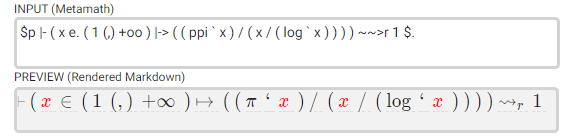
\includegraphics[height=3cm]{formal}}
\caption{The prime number theorem written in Metamath language and rendered as Markdown in real time.}
\label{formal}
\end{center}
\end{figure}

\subsection{\LaTeX\space Support}

While multiple applications extend Markdown to support TeX, there is no standardized syntax specification. However, Pandoc is the most widely used tool for converting \LaTeX\space to Markdown, and its specification is well documented and tested. Thus, we use their specification for our extension \cite{pandoc}:

\blockquote{Anything between two \$ characters will be treated as TeX math. The opening \$ must have a non-space character immediately to its right, while the closing \$ must have a non-space character immediately to its left, and must not be followed immediately by a digit. Thus, \$20,000 and \$30,000 won’t parse as math. If for some reason you need to enclose text in literal \$ characters, backslash-escape them and they won’t be treated as math delimiters.

For display math, use \$\$ delimiters. (In this case, the delimiters may be separated from the formula by whitespace. However, there can be no blank lines between the opening and closing \$\$ delimiters.)}

The following example summarizes the specification:
\begin{quote}
\begin{verbatim} 
Einstein's most famous equation is $E=mc^2$ but it is his handwritten theory of 
happiness is what fetched $1.3 million recently. While it may not fetch many \$s, I 
like the field equations more: $$G_{\mu \nu }+\Lambda g_{\mu \nu }=\kappa T_{\mu \nu }$$
\end{verbatim}
\end{quote}


The above Markdown code is rendered as:
\begin{mdframed}
Einstein's most famous equation is $E=mc^2$ but it is his handwritten theory of happiness is
what fetched \$1.3 million recently. While it may not fetch many \$s, I like the field
equations more: $$G_{\mu \nu }+\Lambda g_{\mu \nu }=\kappa T_{\mu \nu }$$
\end{mdframed}

\section{Sophize Collaboration [From CICM]}

Sophize's communication interface is designed to allow multiple researchers to collaboratively solve a problem. In such open online collaborations, a lot of different ideas and approaches get introduced rapidly. Going through all these comments and making sense of the rapidly evolving ideas becomes a daunting task that can dissuade even the experts and the highly motivated. We believe that we have created a novel interface that can significantly mitigate this problem. The work is primarily influenced by recommendations made by Timothy Gowers and Terence Tao after organizing several Polymath projects \cite{polymath_blog}. We believe that the interface can aid many collaboration types - with few or many participants. We demonstrate the various features of this interface by incorporating actual data from a Polymath project at: \url{https://youtu.be/d3gaalJ7UQM}.

\begin{figure}[ht]
\begin{center}
\fbox{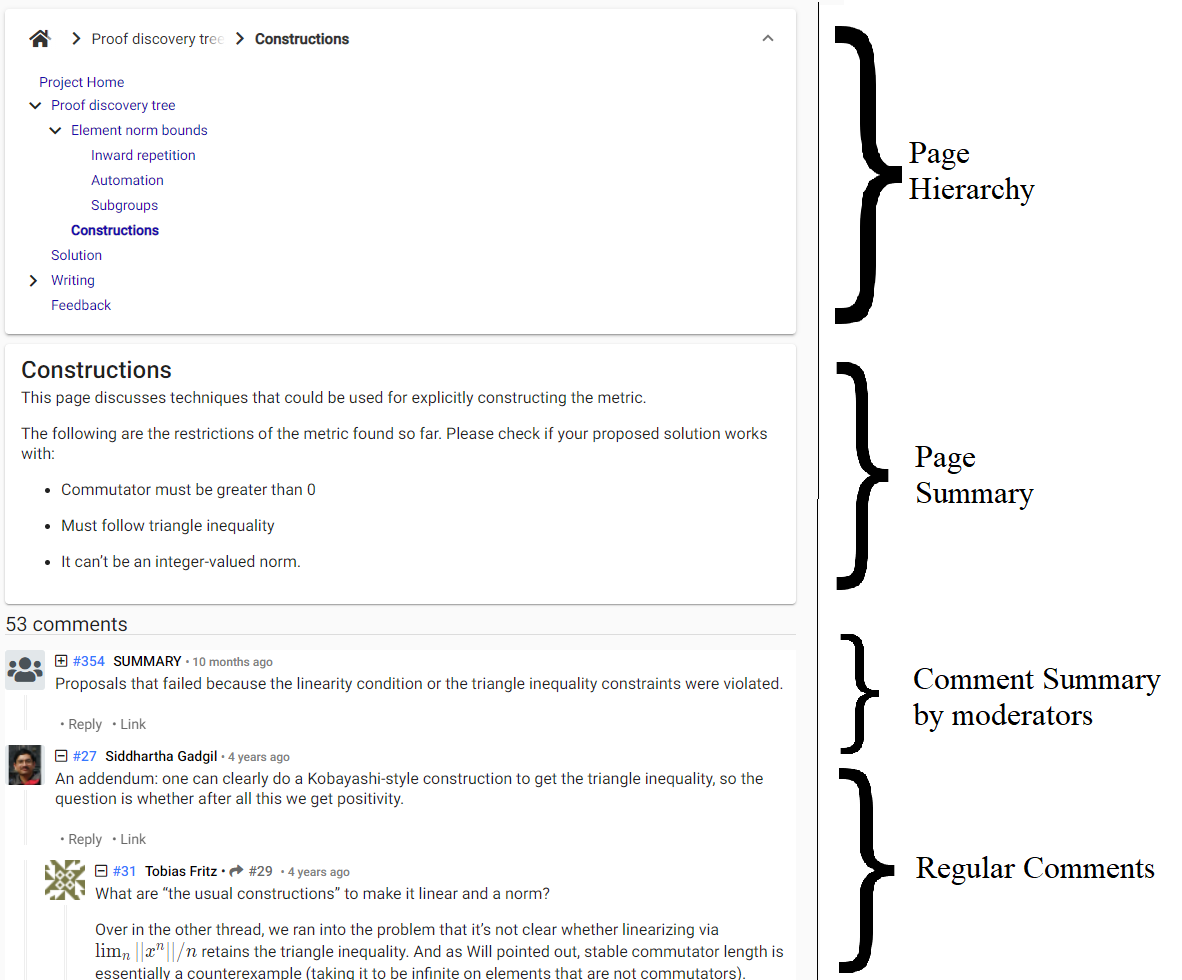
\includegraphics[height=14cm]{collab}}
\caption{Some elements of the Sophize Collaboration Interface.}
\label{collab}
\end{center}
\end{figure}

\subsubsection*{Requirements}

Helping users make sense of the conversation and allowing them to get up to speed with existing progress as quickly as possible is perhaps the most important requirement for managing online collaborations. To solve this problem, we need to organize the ideas in an intuitive way and to summarize the progress. A reader should be able to quickly grasp the current state, and project moderators need a way to manage the direction of various threads to avoid the big picture from being obscured.

Other technical requirements were discussed by some project participants and summarized by Tao on his blog \cite{whats_new_2009} (lightly edited):

\begin{itemize}

  \item \LaTeX\space support

  \item Group moderation

  \item Comment editing and preview

  \item Comment numbering and/or threading

  \item Wiki-like features, i.e., group-editable, publicly-viewable documents with version control

  \item Some way to view all recent comments or developments in a project

  \item Easy registration process

  \item Easy commenting process (i.e., no technical knowledge required)

  \item Permanent URLs for posts and comments (for link-back purposes)

\end{itemize}


We note that Sophize provides all the above features except that it doesn't yet allow users to look at the previous versions of documents. We summarize innovative features of the platform below:

\subsection{Hierarchical Page Organization}

As noted by Gowers, to make sense of the numerous ideas discussed, they need to be organized in a natural hierarchical way. The `proof discovery tree', as described by Gowers \cite{gowers_weblog_2009}, would have a precise approach to the main problem, and each of the subproblems that come up would have its own trees. The leaves of the tree would thus be sub-problems that get solved without division into sub-problems.

Sophize brings the `Proof-discovery tree' to life by organizing the project using neatly organized wiki-like pages. Pages have a parent-child relationship allowing them to be organized like a tree. Discussion comments can be posted on any page, and moderators can rearrange them the way they think is best for the project. Moderators are also encouraged to add an overview on each page that quickly informs readers of the significant ideas that they should be familiar with before they start contributing.

\subsection{Comment Summaries}

Even after the hierarchical division of comments, some pages can still have a large number of comments, which make them difficult to follow. To overcome this problem, we allow project moderators to create summaries of discussions that have taken place so far. Comment summaries get embedded in the comment tree as a parent for comments they summarise. For example, they can club together multiple comment chains that are dead ends so that each reader doesn't waste time on them. Or they could summarize a sub-proof that was arrived at after dozens of comments.

\subsection{Sophize Markdown benefits}

Project collaborators get all the benefits of Sophize Markdown, such as easy linking of existing math content, \LaTeX\space support, and live preview of pages and comments being written or edited.

Comments in Sophize are numbered serially (starting with 1 for each collaboration), each comment can be referenced with the hashtag notation (e.g., `\#3' for the 3rd comment). Comments in an external project can be referenced by providing the project's URI (\#URI/COMMENT\_NUMBER).

Also, we make it extremely easy to extract terms, propositions and proofs from comments. These resources not only help in better understanding of the project, it also helps build Sophize's library.

\subsection{Reducing noise}

Sophize gives project moderators the usual tools like spam removal and fine-grained access control to manage participants. We also add a new feature where certain comments can be marked hidden. Often, threads of dozens of comments can be just noise because they were based on confused concepts or mistaken assumptions. Such comments should not be marked as spam. By marking such threads as `hidden', moderators can ensure that these are not shown by default. But any user can view them when required.

\section{Conclusion and Future Work}

We have presented Sophize Markdown, a lightweight language for representing mathematical knowledge on the web. Using this language, we can easily embed mathematical entities like definitions, theorems, and proofs, making it very convenient to find and browse relevant content. Sophize Markdown plays a central role in organizing proofs from various data sources on the Sophize platform. While there are other ways to represent semantic knowledge, such as content MathML and OpenMath, their scope is somewhat limited to specifying the meaning of the mathematical formula. The sTeX system \cite{Kohlhase2008} is perhaps most similar to Sophize Markdown but it needs creation of \LaTeX\space documents and use of \LaTeX ML systems. This makes its use in real-time web workflows impractical.

We utilized the Sophize Markdown language to create an innovative mathematics communication interface. It is specially designed to aid online mathematics collaborations and can help actualize their vast latent potential. We believe that it can not only aid large-scale collaborations like the Polymath projects but will also be useful for private collaborations and workshops like those organized by AiM.

In the future, we want to make a substantial portion of math literature embedded with structured data available at a much greater scale. Thus, we will improve Sophize Markdown's support for \LaTeX\space features like equation numbering, tables, and references. In addition, we are developing an online tool to easily extract content like definitions, theorems, proofs from math literature by automating some of the tedious tasks. This process will be aided by the recent supervised learning techniques \cite{ginev2019scientific} that classify scientific statements in literature.


\subsection*{Sources}
The Sophize Markdown parser and its Angular renderer source code are available under an MIT license at \url{https://github.com/Sophize/sophize-md-parser} and \url{https://github.com/Sophize/ngx-sophize-md-renderer}, respectively. The NPM packages for these projects are named `sophize-md-parser' and `ngx-sophize-md-renderer'.

\bibliographystyle{alpha} 

\bibliography{mybib}

\end{document}
